\documentclass[12pt, a4paper]{article}

% Idioma e codificação
\usepackage[utf8]{inputenc}
\usepackage[brazil]{babel}

% Layout e margens
\usepackage[top=3cm, bottom=2cm, left=3cm, right=2cm]{geometry}
\usepackage{parskip}
\linespread{1.5}

% Pacotes de matemática
\usepackage{amsmath, amsfonts, amssymb}
\usepackage{mathtools}

% Gráficos, tabelas e elementos flutuantes
\usepackage{graphicx}
\usepackage{float}
\usepackage{caption}
\usepackage{pdflscape}
\usepackage{caption}
\usepackage{subcaption}

% Listagem de código e gestão de cores
\usepackage{listings}
\usepackage{color}

% Diversos
\usepackage{enumitem}
\usepackage{indentfirst}
\usepackage{authblk}
\usepackage{hyperref}
\usepackage{booktabs}

\lstset{
    language= Python,
    basicstyle=\ttfamily\small,
    aboveskip={1.0\baselineskip},
    belowskip={1.0\baselineskip},
    columns=fixed,
    extendedchars=true,
    breaklines=true,
    tabsize=4,
    prebreak=\raisebox{0ex}[0ex][0ex]{\ensuremath{\hookleftarrow}},
    frame=lines,
    showtabs=false,
    showspaces=false,
    showstringspaces=false,
    keywordstyle=\color[rgb]{0.627,0.126,0.941},
    commentstyle=\color[rgb]{0.133,0.545,0.133},
    stringstyle=\color[rgb]{01,0,0},
    numbers=left,
    numberstyle=\small,
    stepnumber=1,
    numbersep=10pt,
    captionpos=t,
    escapeinside={\%*}{*)}
}

%%%%%%%%%%%%%%%%%%%%%%%%%%%%%%%%%%%%%%%%%%%%%%%%%%%%%%%%%%%%%%%%%%%%%%%%%%%%%%%%%

\title{Uma análise numérica do atrator de Lorenz\\ \large{MAP2310 — Métodos
        Numéricos em Equações Diferenciais I \\ }}
\author{Lucas Amaral Taylor}
\affil{Instituto de Matemática e Estatística, Universidade de São Paulo - USP}
\author{Julio Cezar de Moura Lima}
\affil{Instituto de Matemática e Estatística, Universidade de São Paulo - USP}
\begin{document}

\maketitle

%%%%%%%%%%%%%%%%%%%%%%%%%%%%%%%%%%%%%%%%%%%%%%%%%%%%%%%%%%%%%%%%%%%%%%%%%%%%%%%%%
%%%%%%%%%%%%%%%%%%%%%%%%%%%%%%%%%%%%%%%%%%%%%%%%%%%%%%%%%%%%%%%%%%%%%%%%%%%%%%%%%

\begin{abstract}
    No presente relatório aplicaremos os métodos numéricos estudados na
    disciplina
    MAP2310 no sistema de equações diferenciais do atrator de Lorenz.

    \vspace{0.25cm}

    \noindent \textbf{Palavras-chave:} Métodos numéricos; Atrator de Lorenz;
\end{abstract}

%%%%%%%%%%%%%%%%%%%%%%%%%%%%%%%%%%%%%%%%%%%%%%%%%%%%%%%%%%%%%%%%%%%%%%%%%%%%%%%%%
%%%%%%%%%%%%%%%%%%%%%%%%%%%%%%%%%%%%%%%%%%%%%%%%%%%%%%%%%%%%%%%%%%%%%%%%%%%%%%%%%

\section{Introdução}\label{introdução}

Edward Norton Lorenz (1917–2008) foi um matemático e meteorologista que
realizou uma grande contribuição para o estudo de previsões meteorológicas
utilizando-se equações diferenciais. O \textbf{Atrator de Lorenz }foi uma das
principais contribuições do matemático nesta área de estudo. Publicado na
revista \textit{Journal of the Atmospheric Sciences} em 1963 com o título
\textit{Deterministic Nonperiodic Flow} \cite{Lorenz1963}, Lorenz desenvolveu
um modelo matemático simplificado para convecção atmosférica de três equações
diferenciais ordinárias expressas abaixo:

\begin{align}
    \begin{cases}
        \dfrac{dx}{dt} & = \sigma(y-x)     \\
        \dfrac{dy}{dt} & = x(\rho - z) - y \\
        \dfrac{dz}{dt} & = xy - \beta z
    \end{cases}
    \label{eq:apresentacao-sistema}
\end{align}

Além da clara importância do modelo para a meteorologia, o modelo é
conhecido por ser caótico e inaugurar o estudo da Teoria do Caos.

Neste relatório, assim como Edward Norton Lorenz, Ellen Cole Fetter Gille e
Margaret Elaine Hamilton — estas duas importantes matemáticas que contribuíram
com o trabalho de Lorenz — faremos simulações numéricas para estudar o sistema
de equações expostas em \eqref{eq:apresentacao-sistema}.

Logicamente, com a diferença de ser em um nível de graduação e, assim como
orientado, utilizando o conteúdo aprendido em aula. Para tal tarefa, seguiremos
a seguinte abordagem: primeiro, usaremos o método \textit{Runge-Kutta} para
discretizar e resolver o sistema de equações diferenciais que define o atrator.
Em seguida, para a representação gráfica, utilizaremos o \textit{splines}
cúbicas. O atrator de Lorenz tem curvas suaves e acreditamos que essa seja o
melhor método para isso. Por fim, usaríamos o Método dos Mínimos Quadrados
(MMQ) para ver a sensibilidade do sistema (o sistema é conhecido por ser bem
sensível). Com o MMQ criaremos um conjunto de simulações com variações leves em
cada um dos parâmetros e comparamos ao final.

\newpage
\section{Modelagem Matemática}
Nesta seção, apresentaremos considerações e premissas que levam à equação
diferencial que modela matematicamente. Além disso, mostraremos como o sistema
de equações é consistente em relação ao Problema de Cauchy e, ao final,
apresentaremos as condições iniciais e o domínio de definição do problema.

\subsection{Considerações e premissas}

Na introdução de seu artigo, Lorenz afirma que o sistema de equações
expostos em \eqref{eq:apresentacao-sistema} é um modelo determinístico de
sistemas hidrodinâmicos ideais e que tais sistemas foram desenvolvidos para
representar sistema hidrodinâmico dissipativo de força. Além disso, cabe
destacar que que o trabalho do artigo de \textit{Deterministic Nonperiodic
    Flow}\cite{Lorenz1963}, tem como principal base o artigo \textit{Finite
    Amplitude Free Convection as an Initial Value Problem—I} publicado em 1962
de
autoria de Barry Saltzman \cite{Saltzman1962}.

A partir do artigo de Saltzman, introduziremos ao leitor os conceitos
meteorológicos, metodologia utilizada pelo autor e, por fim, o raciocínio
matemático para chegar nas equações propostas por Saltzman até o sistema de
equações de \eqref{eq:apresentacao-sistema} trabalhados por Lorenz. Os detalhes
do desenvolvimento da equação podem ser consultados pelo leitor nos artigos
citados \cite{Lorenz1963} e \cite{Saltzman1962}.

Antes de iniciar, é necessário explicar o que seria o fenômeno de
convecção. Convecção é um processo de transferência de calor que ocorre em
fluidos, como líquidos e gases. Esse fenômeno envolve o movimento do próprio
fluido, transferindo energia térmica de uma região para outra.

Em \cite{Saltzman1962}, o autor como base experimentos meteorológicos e
hidrodinâmicos. Neles, os pesquisadores trabalham com modelos de um fenômeno de
convecção de natureza não-linear, devido às variações espaciais de movimento e
temperatura. Saltzman tem dois objetivos: formular um modelo matemático e um
método de solução de um caso de movimento convectivo dependente do tempo
bidimensionais. Para isso, ele utiliza um número fixo e limitado de componentes
de Fourier e resultados de trabalhos precedentes, destacando-se: \textit{On
    convection currents in a horizontal layer of fluid, when the higher
    temperature
    is on the under side} \cite{Rayleigh1916} e \textit{Ueber die Wärmeleitung
    der
    Flüssigkeiten bei Berücksichtigung der Strömungen infolge von
    Temperaturdifferenzen} \cite{Oberbeck1879}.

Após manipulações algumas manipulações algébricas, cujo leitor pode
conferir os detalhes em \cite{Saltzman1962}, Saltzman chega ao seguinte sistema
de equações diferencias:

\begin{align}
    \frac{\partial}{\partial t} \nabla^2 \psi & = - \frac{\partial (\psi,
        \nabla^2 \psi)}{\partial (x,z)} + v \nabla^4 \psi + g \alpha
    \frac{\partial
    \theta}{\partial x} \label{saltzman-1}                                \\
    \frac{\partial}{\partial t} \theta        & = \frac{\partial (\psi,
        \theta)}{\partial (x,z)} + \frac{\Delta T}{H} \frac{\partial
        \psi}{\partial x}
    + \kappa \nabla^2 \theta \label{saltzman-2}
\end{align}

Onde:
\begin{itemize}
    \item $\psi$: função de fluxo bidimensional ($m^2 \cdot s^{-1}$)
    \item $\theta$: desvio de temperatura ($K$);
    \item $g$: aceleração da gravidade ($m \cdot s^{-2}$);
    \item $\alpha$: coeficiente de expansão térmica ($K^{-1}$);
    \item $v$: constante de viscosidade cinemática ($m^2 \cdot s^{-1}$);
    \item $\kappa$: constante de condutividade térmica ($W \cdot m^{-1}
              \cdot K^{-1}$).
\end{itemize}

Manipulando os termos e adicionando os componentes de Fourier, obtemos a
seguinte expressão \cite{peitgen2013} \cite{Saltzman1962}:
\begin{align}
    \frac{a}{(1 + a^2)^k} \psi        & = x(t)\sqrt{2} \sin \left(\frac{\pi
    u}{a}\right) \sin \left(\frac{\pi v}{H}\right) \label{saltzman-forier-1} \\
    \frac{\pi R_o \theta}{R \Delta T} & = y(t)\sqrt{2} \cos \left(\frac{\pi
        u}{a}\right) \sin \left(\frac{\pi v}{H}\right)
    \label{saltzman-forier-2} - z(t)
    \sin \left(\frac{2\pi}{H}v\right)
\end{align}

Onde:
\begin{itemize}
    \item $u$: coordenada espacial horizontal ($m$);
    \item $x(t), y(t), z(t)$: coeficientes dependentes do tempo
          (amplitudes) (Unidade depende do contexto);
    \item $\frac{\pi}{H}$: inverso da profundidade da camada de fluido
          (máximo de $v$) ($m^{-1}$);
    \item $a$: parâmetro de geometria;
    \item $Ra$: número de Rayleigh \cite{Rayleigh1916};
    \item $R_c$: valor crítico de $Ra$ ($R_c = \pi^4(1 + a^2)^3/a^2$);
    \item $\Delta T$: diferença de temperatura total ($K$).
\end{itemize}

Finalmente, em posse de todas essas equações. Realizando a substituição de
\ref{saltzman-forier-1} e \ref{saltzman-forier-2} em \ref{saltzman-1} e
\ref{saltzman-2} e eliminando as funções trigonométricas, obtemos
\ref{eq:apresentacao-sistema}, isto é:

\begin{align*}
    \begin{cases}
        \dfrac{dx}{dt} & = \sigma(y-x)     \\
        \dfrac{dy}{dt} & = x(\rho - z) - y \\
        \dfrac{dz}{dt} & = xy - \beta z
    \end{cases}
\end{align*}

\begin{itemize}
    \item $\sigma$ controla a sensibilidade do sistema à diferença entre as
          variáveis $x$ e $y$ (número de Prandtl).

    \item $\rho$ está associado à taxa de convecção do sistema.(número de
          Rayleigh)

    \item $\beta$ está associado à geometria do sistema e à diferença entre
          as taxas de crescimento das variáveis $x$ e $z$.

\end{itemize}

\subsection{O problema de Cauchy}
Lorenz em seu artigo, considera o sistema de equações como um sistema
dissipativo de energia composto por um conjunto finito de equações lineares em
um espaço de fase.

\subsubsection{Um sistema dissipativo em um espaço de fase}

Primeiramente, é importante definir o que é um sistema dissipativo de
energia e o que é um espaço de fase e como estes conceitos dialogam com o
atrator de Lorenz.

Sistemas dissipativos de energia tem como característica o fato de perder
energia em processos não conservativos, como atrito, transformando-se em formas
menos úteis, como calor. O Atrator de Lorenz é um exemplo desses sistemas, por
se tratar do fenômeno convecção atmosférica (fenômeno devidamente explicado na
seção anterior), onde a energia constantemente alimentada e dissipada.

O espaço de fase é uma representação que descreve todos os possíveis
estados de um sistema dinâmico através de suas variáveis. Cada ponto neste
espaço indica um estado específico do sistema.

Isto posto, podemos explicar a abordagem tomada por Lorenz para explicar a
existência e unicidade da equação diferencial. Podemos classificar o fenômeno
de convecção como um sistema dissipativo de energia formado por conjunto finito
de equações lineares. Isto posto, podemos tomar $n$ variáveis $x_1, \ldots,
    x_n$ e definir o seguinte sistema:
\begin{equation}
    \frac{dx_i}{dt} = F_i\left(x_1, \ldots, x_n\right) \quad i \in \{1,
    \ldots, n\}
\end{equation}

Onde $F_i$ possui derivadas parciais de primeira ordem contínuas e $t$ é a
única variável independente. Assim, para descrever todos os possíveis estados
de um sistema dinâmico através de suas variáveis, adequaremos o sistema em um
espaço de fase euclidiano de dimensão $n$ constituído pelas variáveis $x_1,
    \ldots, x_n$.

Assim, como o sistema é composto por equações lineares com variáveis
dependentes e que $F_i \in C_1$, temos que, consequentemente, o sistema possui
solução única diretamente. Isto é:
\begin{equation}
    x_i = f_i(x_{1_0}, \ldots, x_{n_0}, t) \quad i = \{1, \ldots, n\}
\end{equation}

Para algum intervalo que contenha $t_0$ e satisfaça a condição abaixo:
\begin{equation*}
    f_i(x_{1_0}, \ldots, x_{n_0}, t_0) = x_{i_0} \quad i = \{1, \ldots,
    n\}
\end{equation*}

Tal fato é demonstrado em \cite{ford1933} na forma de um Teorema, exposto a
seguir:

\textbf{Teorema.} Considere um intervalo fechado $[A, B]$ onde as funções
$F_i(x_1, \ldots, x_n)$ são contínuas juntamente com suas derivadas parciais de
primeira ordem $\frac{\partial F_i}{\partial x_j}$ para todos $1 \leq i,j \leq
    n$. Se para algum ponto $t_0$ em $(A, B)$ são dadas condições iniciais
$x_{i_0}
    = x_i(t_0)$, então existe um único conjunto de funções $x_i(t)$ que são
soluções do sistema no intervalo $[A, B]$ e satisfazem $x_i(t_0) = x_{i_0}$.
Além disso, as soluções $x_i(t)$ possuem derivadas contínuas em $[A, B]$.

Com base no teorema apresentado e na formulação das equações diferenciais
$\frac{dx_i}{dt} = F_i(x_1, \ldots, x_n)$, o problema de \textit{Cauchy} é
adequadamente satisfeito. Dadas condições iniciais em um tempo $t_0$, a
existência e unicidade das soluções $x_i(t)$ são garantidas para o intervalo
$[A, B]$.

\subsubsection{Uma breve nota do Teorema da Existência e Unicidade de
    Picard}
Primeiramente, expressaremos o Teorema da Existência e Unicidade de Picard
utilizando a \cite{sotomayor1979}:

\textbf{Teorema.}Seja $f$ contínua e lipschitzana em $\Omega = I_a \times
    B_b$, onde $I = \{t; \left|t - t_0 \right| \leq a\}$, $B_b = \{x; \left|x -
    x_0
    \right| \leq b\}$. Se $|f| \leq M$ em $\Omega$, existe uma e única solução
de

\begin{equation*}
    x^\prime = f(t, x), \quad x(t_0) = x_0
\end{equation*}

em $I_\alpha$ onde $\alpha = \min \{a, b/M\}$

Geralmente, a fim de mostrar a resolução do problema de \textit{Cauchy},
utiliza-se como abordagem o Teorema exposto acima. Este método não foi
utilizado para a tratar o sistema de Lorenz.

Ao pesquisar livros e referências sobre o tema, nenhum utilizou como
abordagem este método. Isso porque é fácil de demonstrar que as funções do
sistema \eqref{eq:apresentacao-sistema} tem derivada contínua, mas pelo sistema
ser não-linear a demonstração de ser localmente lipschitzana é extremamente
complexa e é preferível a abordagem utilizada pelo próprio autor em
\cite{Lorenz1963}. Optamos por seguir a abordagem majoritariamente utilizada.

\subsubsection{Condições iniciais e domínio de definição do problema}
\label{sec:cond-ini}
Definiremos o domínio de definição do problema da seguinte forma: as
variáveis $x,y, z \in \mathbb{R}$ refletindo a capacidade do sistema de atingir
qualquer estado no espaço tridimensional (cabe dizer aqui que: apesar de Lorenz
tratar o sistema em um estado de fase, por questões de simplicidade e
representação computacional clara, utilizaremos o espaço tridimensional em
nossas simulações). Além disso, temos que $t \in [0, \infty)$, o tempo começa
em zero e não tem limite superior, permitindo a análise do sistema ao longo do
tempo para observar seu comportamento dinâmico.

As condições iniciais que definimos são: $\sigma = 10$, $\rho = 28$ e
$\beta = \frac{8}{3}$. Os valores apresentados são tipicamente escolhidos em
simulações da literatura. Além disso, as escolhas de $x$, $y$ e $z$ são números
reais arbitrariamente escolhidos, por questões de simplicidade escolheremos: $x
    = 0$, $y=1.0$ e $z=1.05$.
\newpage

%%%%%%%%%%%%%%%%%%%%%%%%%%%%%%%%%%%%%%%%%%%%%%%%%%%%%%%%%%%%%%%%%%%%%%%%%%%%%%%%%
%%%%%%%%%%%%%%%%%%%%%%%%%%%%%%%%%%%%%%%%%%%%%%%%%%%%%%%%%%%%%%%%%%%%%%%%%%%%%%%%%

\section{Metodologia Numérica}
Nesta seção, apresentaremos os métodos utilizados no desenvolvimento do
trabalho, justificando devidamente o emprego de cada uma. A fim de promover uma
descrição adequada de cada método utilizaremos como referência \cite{roma2023}
e \cite{burden2016}.

\subsection{Uma breve nota sobre os métodos utilizados}
Nesta seção, apresentamos os métodos numéricos de maneira teórica,
detalhando as justificativas e o funcionamento teórico conforme a abordagem
adotada durante as aulas. É importante ressaltar que, na aplicação prática,
utilizamos as bibliotecas \textit{numpy} e \textit{scipy} na linguagem de
programação \textit{Python}. Optamos por não incluir no texto algumas
divergências e detalhes específicos relacionados ao uso dessas ferramentas
computacionais, pois eles se referem mais à implementação técnica nas
bibliotecas e as especificações delas do que aos conceitos teóricos discutidos
em aula.

\subsection{Método Runge-Kutta}
\subsubsection{Justificativa da escolha do método}
O fato do atrator de \textit{Lorenz} ser um sistema não linear, de alta
sensibilidade, principalmente, pela mudança das condições iniciais, e caótico.
Pelo fato calcular as inclinações em quatro pontos dentro de cada intervalo de
tempo, o método oferece uma aproximação mais precisa comparada aos demais
aprendidos em aula. Por exemplo, o método de Euler não seria suficientemente
eficaz para a discretização do sistema por não modelar muito bem fenômenos de
natureza não linear. A

Além disso, O Runge-Kutta de quarta ordem, oferece um erro de
truncamento local da ordem de $h5$ e um erro de truncamento global da ordem de
$h4$, onde $h$ é o passo de tempo \cite{burden2016} \cite{roma2023}. Isso
significa que pequenos aumentos no passo de tempo podem produzir resultados
precisos sem aumentar significativamente o erro, o que é ideal para lidar com a
dinâmica complexa e sensível do atrator de Lorenz.

\subsubsection{Funcionamento do método}
O método Runge-Kutta visa discretizar os valores do sistema
\eqref{eq:apresentacao-sistema} com os valores iniciais apresentados na seção
\ref{sec:cond-ini}. Seguiremos o método apresentado em \cite{roma2023}:

\begin{equation}
    \Phi(t, y, h) = \frac{1}{6} (\kappa_1 + 2\kappa_2 + 2\kappa_3 +
    \kappa_4)
\end{equation}

De tal forma que:
\begin{align}
    \begin{cases}
        \kappa_1 = f(t, y)         \\
        \kappa_2 = f\left(t + \frac{h}{2}, y +
        \frac{h}{2}\kappa_1\right) \\
        \kappa_3 = f\left(t + \frac{h}{2}, y +
        \frac{h}{2}\kappa_2\right) \\
        \kappa_4 = f(t + h, y + h\kappa_3)
    \end{cases}
\end{align}

\subsection{\textit{Spline} Cúbico}
\subsubsection{Justificativa da escolha do método}
Utilizaremos o método de interpolação chamado \textit{spline} cúbico. A
escolha deste método para a interpolação dos dados do atrator de Lorenz é
motivada pela necessidade de representar as curvas do sistema de maneira suave
e contínua, uma característica crucial para tratar sua natureza não-linear e
caótica.

Outros métodos, como, por exemplo, o método de interpolação de Lagrange
não seria adequado, já que este envolve um processo de linearização que
acarretaria perda de informação e, consequentemente, não representaria o
sistema da melhor forma possível.

\subsubsection{Funcionamento do método}
Este método envolve a criação de um polinômio cúbico em cada subintervalo
de um intervalo total, para interpolar um conjunto de pontos dados. Seguiremos
como referência a construção de \textit{spline} proposta pela referência
\cite{burden2016}, expressa abaixo:

Seja $f$ uma função definida no intervalo $[a,b]$ e $ \{a = x_0 < x_1 <
    \ldots < x_n = b\}$ um conjunto de nós. Um interpolante de \textit{spline}
cúbica $S$ para $f$ é uma função que satisfaz as seguintes condições:
\begin{enumerate}
    \item $ S(x) $ é um polinômio cúbico, denotado $ S_j(x) $, em cada
          subintervalo $[x_j, x_{j+1}]$, para $ j = 0, 1, \ldots, n-1 $.
    \item $ S_j(x_j) = f(x_j) $ e $ S_j(x_{j+1}) = f(x_{j+1}) $ para cada $
              j = 0, 1, \ldots, n-1 $.
    \item $ S_{j+1}(x_{j+1}) = S_j(x_{j+1}) $ para cada $ j = 0, 1, \ldots,
              n-2 $.
    \item $ S'_{j+1}(x_{j+1}) = S'_j(x_{j+1}) $ para cada $ j = 0, 1,
              \ldots, n-2 $.
    \item $ S''_{j+1}(x_{j+1}) = S''_j(x_{j+1}) $ para cada $ j = 0, 1,
              \ldots, n-2 $.
    \item Uma das seguintes condições de contorno é satisfeita:
          \begin{enumerate}
              \item $S''(x_0) = S''(x_n) = 0$ (contorno livre ou natural).
              \item $S'(x_0) = f'(x_0)$ (contorno fixado ou clampeado).
          \end{enumerate}
\end{enumerate}

\subsection{Método dos Mínimos Quadrados}
\subsubsection{Justificativa da escolha do método}
Utilizamos o Método dos Mínimos Quadrados (MMQ) para analisar a
sensibilidade do atrator de Lorenz ao longo do tempo. Embora o atrator de
Lorenz seja um sistema altamente não-linear, o MMQ proporciona uma boa
aproximação das dinâmicas envolvidas nesse sistema. Além disso, ele quantifica
o impacto das alterações em cada parâmetro, evidenciando como pequenas mudanças
nas variáveis podem afetar o sistema. Por fim, vale destacar a alta eficiência
computacional deste método.

\subsubsection{Funcionamento do método}
O método dos mínimos quadrados polinomial aproxima um conjunto de dados
$(x_i, y_i)$, com um polinômio algébrico $P_n(x)$ de grau $n < m - 1$,
escolhendo os coeficientes $a_0, a_1, \ldots, a_n$ para minimizar o erro
quadrático $E = \sum_{i=1}^m (y_i - P_n(x_i))^2$. Isso resulta em $n + 1$
equações normais para os $n + 1$ coeficientes desconhecidos $a_j$:

\begin{equation}
    \sum_{k=0}^n a_k \left(\sum_{i=1}^m x_i^{j+k}\right) = \sum_{i=1}^m y_i
    x_i^j, \quad \text{para cada } j = 0, 1, \ldots, n.
\end{equation}

Resolvendo esse sistema, obtemos os coeficientes do polinômio que melhor se
ajusta aos dados no sentido dos mínimos quadrados. A ser expresso em:
\begin{equation*}
    P_n(x) = a_nx^n + a_{n-1}x^{n-1} + \cdots + a_1x + a_0
\end{equation*}

Detalhes a serem vistos em \cite{burden2016}.
\newpage

%%%%%%%%%%%%%%%%%%%%%%%%%%%%%%%%%%%%%%%%%%%%%%%%%%%%%%%%%%%%%%%%%%%%%%%%%%%%%%%%%
%%%%%%%%%%%%%%%%%%%%%%%%%%%%%%%%%%%%%%%%%%%%%%%%%%%%%%%%%%%%%%%%%%%%%%%%%%%%%%%%%


\section{Metodologia Computacional}
A fim de aplicar os métodos citados anteriormente, essa seção traz como
proposta apresentar a abordagem computacional no emprego dos métodos,
comprovação do comportamento no fenômeno de atrator e por fim avaliar algumas
métricas provenientes de cada uma das metodologias.

\subsection{Contexto}
Apresentamos métodos de ``discretização'' que possibilitam estimar valores
para o vetor solução $S = \begin{bmatrix} x(t) \\ y(t) \\ z(t)\end{bmatrix}$ em
um dado tempo $t$. Durante a metodologia computacional os passos trabalhados
foram:
\begin{enumerate}
    \item Aplicação de Runge-Kutta no sistema de Lorenz com $n\_steps =
              10^4$, ou seja, o vetor solução seria calculado ao longo de 10
          000 períodos. A
          justificativa para a quantidade de pontos é dada graficamente, de
          modo que o
          atrator toma forma ao longo do tempo.
    \item A partir das soluções encontradas em RK, os dados são tabelados e
          assim utilizados para interpolação \textit{spline} cúbica. De maneira
          análoga,
          para MMQ, portanto, teremos dois polinômios interpoladores.
    \item Com os polinômios previamente calculados desenhos os gráficos.
\end{enumerate}

\subsection{Dados preliminares}
Utilizando o método RK, três simulações foram feitas para o sistema de
Lorenz já definido, mostrando que o fenômeno atrator forma as espirais conforme
os passos dados, sabendo que um tempo($t$) maior gera com mais assertividade o
fenômeno evidenciado por Lorenz(\textit{Visualização na figura 3}).

A função em \textit{Python} responsável por calcular RK é definida pelos
seguintes parâmetros: $\sigma,\ \rho,\ \beta, x_0, y_0, z_0, h, num\_steps$.
Considerando as variáveis comuns ao sistema convencionado, sendo $(x_0,\ y_0,\
    z_0)$ condições iniciais do sistema e $h$ o comprimento do intervalo em que
$t$(tempo) está compreendido.

Na execução da função, valores comuns dentro do estudo de Lorenz foram
usados, de modo que:
\begin{equation}
    \begin{aligned}
        \sigma            & = 10,          \\
        \rho              & = 28,          \\
        \beta             & = \frac{8}{3}, \\
        x_0               & = 0,           \\
        y_0               & = 1,           \\
        z_0               & = 1.05,        \\
        h                 & = 0.01,        \\
        \text{num\_steps} & = 10^4
    \end{aligned}
\end{equation}

\begin{table}[H]
    \centering
    \begin{tabular}{|c|c|c|c|c|}
        \hline
        Índice & X        & Y        & Z        \\
        \hline
        0      & 0.000000 & 1.000000 & 1.050000 \\
        1      & 0.095105 & 1.003039 & 1.022849 \\
        2      & 0.182649 & 1.030512 & 0.997333 \\
        3      & 0.265581 & 1.080595 & 0.973428 \\
        4      & 0.346436 & 1.152210 & 0.951187 \\
        5      & 0.427432 & 1.244918 & 0.930735 \\
        6      & 0.510567 & 1.358849 & 0.912268 \\
        7      & 0.597683 & 1.494637 & 0.896062 \\
        8      & 0.690531 & 1.653393 & 0.882484 \\
        9      & 0.790823 & 1.836671 & 0.872011 \\
        10     & 0.900278 & 2.046464 & 0.865257 \\
        11     & 1.020660 & 2.285199 & 0.863005 \\
        12     & 1.153819 & 2.555743 & 0.866250 \\
        13     & 1.301723 & 2.861417 & 0.876253 \\
        14     & 1.466492 & 3.206010 & 0.894607 \\
        15     & 1.650427 & 3.593802 & 0.923322 \\
        \hline
    \end{tabular}
    \caption{Seleção de 15 pontos}
\end{table}

\begin{figure}[H]
    \centering
    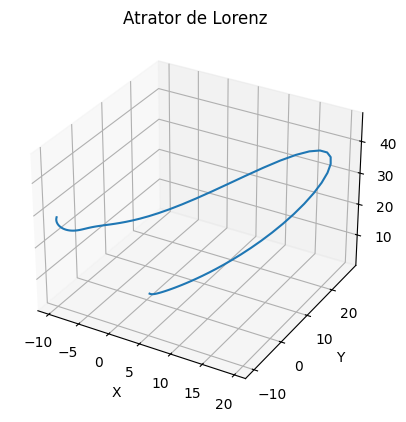
\includegraphics[width=0.5\textwidth]{img/attrator100.png}
    \caption{Atrator para 100 passos.}
    \label{fig:lorenz102}
\end{figure}

\begin{figure}[H]
    \centering
    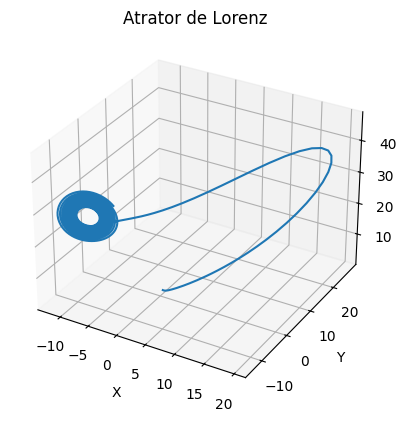
\includegraphics[width=0.5\textwidth]{img/attrator1000.png}
    \caption{Atrator para 1000 passos.}
    \label{fig:lorenz103}
\end{figure}

\begin{figure}[H]
    \centering
    \includegraphics[width=0.5\textwidth]{img/attrator10000.png}
    \caption{Atrator para 10000 passos.}
    \label{fig:lorenz104}
\end{figure}

\subsection{Métodos Interpoladores}
\subsubsection{\textit{Spline} Cúbica}

No emprego do método de interpolação por \textit{spline} cúbica foi
utiliza a biblioteca \href{https://docs.scipy.org/doc/scipy/index.html}{Scipy}
do python, sendo aplicado o método $scipy.interpolate.CubicSpline$. O motivo
por tal técnica é para fins de teste e comprovação do método, dado que o número
de pontos trabalhados é alto, o que gera um custo computacional significativo.
Observando o método, vemos que a estratégia segue algo que Lorenz já evidenciou
nos testes, assim sendo um bom método interpolador que compreende o
comportamento ``oscilante'' descrito no problema.

\begin{figure}[H]
    \centering
    \includegraphics[width=\textwidth]{img/spline.png}
    \caption{Spline Cúbica}
    \label{fig:spline}
\end{figure}

\subsubsection{MMQ}
Já no MMQ, seguimos a mesma estratégia abordada na \textit{spline}
cúbica, mas com o pacote \href{https://numpy.org/doc/stable/index.html}{NumPy}
e para biblioteca $numpy.polyfit$, de modo que o pacote faça um \textit{fit}
através da estratégia de mínimos quadrados com os pontos previamente tabelados.
De fato, não há uma boa predição de dados nas curvas do MMQ, o que se aproxima
do comportamento conhecido de uma regressão linear, já que há uma alta
dispersão nos pontos, grande volume e, por consequência, granularidade na
interpolação.
\begin{figure}[H]
    \centering
    \includegraphics[width=\textwidth]{img/mmq.png}
    \caption{MMQ}
    \label{fig:mmq}
\end{figure}

\newpage

%%%%%%%%%%%%%%%%%%%%%%%%%%%%%%%%%%%%%%%%%%%%%%%%%%%%%%%%%%%%%%%%%%%%%%%%%%%%%%%%%
%%%%%%%%%%%%%%%%%%%%%%%%%%%%%%%%%%%%%%%%%%%%%%%%%%%%%%%%%%%%%%%%%%%%%%%%%%%%%%%%%

\section{Resultados}
\subsection{Análise Manufaturada}

Para realizar a análise de maneira manufaturada, faremos um comparativo intrínseco acerca de um dos métodos que Lorenz abordou na resolução do problema: o método de diferenças progressivas\cite{Lorenz1963} e o método já aprofundado no texto que se trata do RK4.

Como fim didático, vamos detalhar o método de diferenças progressivas(\textit{forward-difference}). A equação que estabelece o método é dada por: 
\begin{equation*}
    X_i(t_{n+1})=X_i(t_n)+F_i(P_n)\Delta t
\end{equation*}
De modo que $F_i(P_n) = \dot X_i(P_n)$ e $t_{n+1} = t_n + \Delta t$, assim fazemos uso de aproximações progressivas, ou seja, diferenças finitas trabalhadas com a função em um tempo $t_n$ e no tempo futuro $t_{n+1}$ para calcular valores futuros.  Abaixo temos a tabela de valores gerada com o método, assim como a diferença entre os valores de cada ponto com os pontos gerados por RK4.

\begin{table}[H]
    \centering
    \begin{tabular}{|c|c|c|c|c|c|c|}
        \hline
         & X & Y & Z & $X-X_{rk}$ & $Y-Y_{rk}$ & $Z-Z_{rk}$ \\
        \hline
        1 & 0.000000 & 1.000000 & 1.050000 & 0.000000 & 0.000000 & 0.000000 \\
        2 & 0.100000 & 0.990000 & 1.022000 & 0.004895 & -0.013039 & -0.000849 \\
        3 & 0.189000 & 1.007078 & 0.995737 & 0.006351 & -0.023434 & -0.001596 \\
        4 & 0.270808 & 1.048045 & 0.971087 & 0.005226 & -0.032550 & -0.002341 \\
        5 & 0.348532 & 1.110761 & 0.948030 & 0.002096 & -0.041449 & -0.003157 \\
        6 & 0.424755 & 1.193938 & 0.926620 & -0.002678 & -0.050980 & -0.004114 \\
        7 & 0.501673 & 1.296994 & 0.906982 & -0.008894 & -0.061854 & -0.005286 \\
        8 & 0.581205 & 1.419943 & 0.889302 & -0.016478 & -0.074694 & -0.006760 \\
        9 & 0.665079 & 1.563312 & 0.873840 & -0.025452 & -0.090081 & -0.008644 \\
        10 & 0.754902 & 1.728089 & 0.860935 & -0.035921 & -0.108582 & -0.011076 \\
        \hline
    \end{tabular}
    \caption{Diferença em comparação com os valores dos pontos de RK4}
    \label{tab:rk44-diff}
\end{table}

Seja $E = \left\{(\mu_x, \mu_y, \mu_z) \in \mathbb{R}^3\right\}$, o vetor de médias amostrais do módulo da diferença entre os pontos. Então $E = (0.007, 0.049, 0.004)$, disso evidenciamos estatisticamente que os pontos gerados não apresentam grandes distâncias, entretanto no caráter de sensibilidade do atrator há grandes mudanças gráficas. Aqui notamos que os saltos em cada iteração são menores, comparados ao RK4, o que reflete diretamente na formação do atrator com `vórtices'' mais compactos e sem grande detalhamento no efeito. Temos a seguinte imagem: 

\begin{figure}[H]
    \centering
    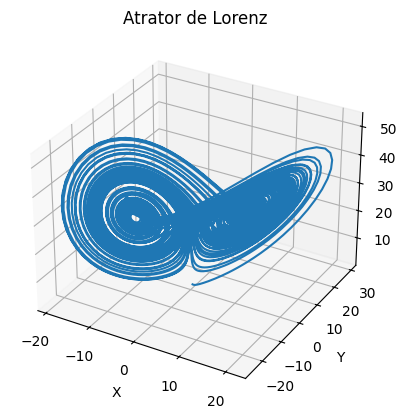
\includegraphics[width=0.4\textwidth]{relatorio/img/attrator10000_lorenz.png}
    \caption{Imagem gerada com método de diferenças progressivas}
    \label{fig:diff-prog}
\end{figure}

\subsection{Aplicações na metereologia}
Como já exposto na introdução deste relatório, podem-se reafirmar a
importância do atrator de Lorenz na meteorologia. Logicamente, apesar de ser um
modelo simplificado daquele exposto por Saltzman em \cite{Saltzman1962}, o
modelo de Lorenz é considerado um ótimo modelo na área para a modelagem de
convecção atmosféricas ao redor do globo.

Um grande exemplo do uso do atrator de Lorenz é o trabalho de Timothy Noel
Palmer intitulado como ``Extended-Range Atmospheric Prediction and the Lorenz
Model'' \cite{Palmer1993}, o qual apresentamos o resumo (em tradução livre)
abaixo:
\begin{quote}
    \fontsize{10}{12}\selectfont
    A base física para a previsão de longo alcance é explorada utilizando o
    famoso modelo de convecção Lorenz de três componentes, tomado como uma
    representação conceitual da circulação extratropical caótica, e alargado
    através do acoplamento a um oscilador linear para representar interações
    tropicais-extratropicais de grande escala. O modelo é utilizado para
    analisar
    os papéis do cálculo da média temporal e da previsão por conjuntos e, numa
    forma alargada, o impacto da temperatura anômala da superfície do mar
    tropical
    e da temperatura anômala da superfície do mar extratropical. Os paradigmas
    conceptuais e os cálculos analíticos apresentados são utilizados para
    interpretar resultados de previsões meteorológicas numéricas e de
    experiências
    com modelos de circulação geral. São apresentadas algumas observações sobre
    a
    relevância dos estudos de previsibilidade para o problema das alterações
    climáticas.
\end{quote}


\newpage

%%%%%%%%%%%%%%%%%%%%%%%%%%%%%%%%%%%%%%%%%%%%%%%%%%%%%%%%%%%%%%%%%%%%%%%%%%%%%%%%%
%%%%%%%%%%%%%%%%%%%%%%%%%%%%%%%%%%%%%%%%%%%%%%%%%%%%%%%%%%%%%%%%%%%%%%%%%%%%%%%%%

\section{Convergência do erro}

A fim de completar nossa análise do atrator de Lorenz, iremos realizar a análise da convergência do erro das duas abordagens trabalhadas no presente relatório. Primeiramente, é importante pontuar que: como o atrator de Lorenz não possui uma solução analítica simples para comparação direta, uma abordagem comum é considerar a solução numérica obtida com o menor $h$ como uma aproximação da solução ``exata''. Então, calcularemos o erro como a diferença entre as soluções numéricas obtidas para os diferentes valores de $h$ e a solução com o menor $h$.

\subsection{Método Runge-Kutta de ordem 4}
\subsubsection{Base teórica}
Para iniciar uma análise comparativa robusta, é essencial primeiro definir e entender as principais características do método utilizado. Com base nessas características, desenvolveremos uma fundamentação teórica sólida que suporte a análise comparativa.

O Método Runge-Kutta de ordem 4, utilizado para a discretização do atrator de Lorenz pelos autores, é um método de passo único, isso porque a solução em cada passo depende apenas do valor da solução no passo anterior, e não de múltiplos passos anteriores. Além disso, é um método de Runge-Kutta explicíto, ou seja, os valores de $k_i$ são calculados diretamente dos valores já conhecidos, sem necessidade de resolver equações adicionais para obter $k_i$

A partir desta caracterização inicial, podemos recorrer a \textbf{Definição 3.1} \cite{roma2023} que lista as três principais propriedades do método RK explícito de ordem $q$ (para o nosso caso, ordem $4$):

\begin{quote}
    \fontsize{10}{12}\selectfont
    \textbf{Definição 3.1} (Propriedades de um RK explícito de ordem $4$). Um método é de \textit{Runge-Kutta explícito de ordem $4$} se, e só se, satisfaz três propriedades:

\begin{enumerate}
    \item é um método de passo único explícito,
    \item tem as derivadas de $y(t)$ (e, portanto, de $D^j f(t,y)$) aproximadas em pontos ``convenientemente escolhidos'' e, por fim,
    \item ``concorda'' com o Método da Série de Taylor até o termo de quarta ordem.
\end{enumerate}
\end{quote}

Após apontar as principais características do método trabalhado, podemos enfim levantar os principais pontos relacionados ao erro do método empregado e sua convergência.

O RK4 usa uma combinação ponderada de quatro inclinações ($\kappa_1, \kappa_2, \kappa_3, \kappa_4$) dentro do intervalo $h$ em pontos específicos para estimar a próxima solução. Ao expandir a solução em série de Taylor e comparar com a fórmula do RK4, pode-se mostrar que os termos de erro de ordem superior são cancelados devido à escolha específica dos coeficientes de ponderação e dos pontos de amostragem. Isso leva a um \textbf{erro local de truncamento de ordem 5} em cada passo. 

Ao acumular os erros locais ao longo de $n$ passos, \textbf{o erro global se torna de ordem 4}, uma ordem a menos. Logo, à medida que o tamanho do passo $h$ diminui, o erro global do RK4 converge para zero\footnote{Por isso, considerar a solução numérica obtida com o menor $h$ como uma aproximação da solução ``exata'' é viável} a uma taxa de $h^4$.

Por fim, a  alta ordem de convergência do RK4 $O(h^4)$ implica que o erro diminui rapidamente à medida que o tamanho do passo $h$ é reduzido. Essa rápida convergência, juntamente com sua natureza explícita e estabilidade numérica, torna o RK4 um método eficiente para o problema trabalhado.


\subsection{Método de diferenças progressivas}
\subsubsection{Base teórica}
O método de diferenças progressivas utilizado como método da análise manufaturado foi o método utilizado pelo Lorenz em \cite{Lorenz1963}. Como devidamente mostrado na seção anterior, temos que ``evidenciamos estatisticamente que os pontos gerados não apresentam grandes distâncias, entretanto no caráter de sensibilidade do atrator há grandes mudanças gráficas''. Essa grande mudança gráfica devido a sensibilidade do sistema será justificada na presente seção. Assim como, o método de Runge-Kutta antes de tratar o erro propriamente, iremos expor propriedades do método a fim de extrair informações mais consistentes e robustas do erro e convergência do método empregado. Isto posto, comecemos nossa análise.

Da maneira que foi empregado, o método de diferenças progressivas pode ser analisado como o método de Euler explícito de passo único. As principais propriedades do método estão listadas a seguir e embasadas pela referência \cite{Fontana2018}:
    \begin{enumerate}
        \item \textbf{Simplicidade:} É um dos métodos mais simples para a resolução de EDOs;
        \item \textbf{Ordem:} É um método de primeira ordem, o que significa que o erro de truncamento é proporcional ao quadrado do tamanho do passo, enquanto o erro acumulado é proporcional ao tamanho do passo;
        \item \textbf{Convergência:} Converge para a solução correta à medida que o tamanho do passo diminui, mas requer passos de tempo pequenos para uma boa precisão, especialmente em sistemas dinâmicos sensíveis;
        \item \textbf{Estabilidade:} Pode ser instável se o passo de tempo não for suficientemente pequeno, o que é crítico em sistemas que são sensíveis às condições iniciais.
    \end{enumerate}

As características do Método de Euler são essenciais para compreender o erro e sua convergência, particularmente quando aplicadas a sistemas complexos como o Atrator de Lorenz. A simplicidade do método, embora benéfica para a implementação, apresenta desvantagens significativas:

\begin{enumerate}
    \item \textbf{Dependência do Tamanho do Passo}: O Método de Euler possui uma alta dependência do tamanho do passo. Isso implica que tanto o erro local quanto o erro global estão diretamente ligados ao tamanho do passo escolhido.

    \item \textbf{Convergência e Estabilidade}: Devido à forte dependência do tamanho do passo, a convergência do método pode ser comprometida. Um passo maior pode resultar em uma solução numérica instável, especialmente em sistemas dinâmicos sensíveis como o Atrator de Lorenz, onde pequenas variações nas condições iniciais podem levar a grandes divergências nas trajetórias calculadas.
\end{enumerate}

Como mencionado anteriormente, o erro local de truncamento para o método de Euler é proporcional ao quadrado do tamanho do passo e o erro global é proporcional ao tamanho do passo. Então:
\begin{equation*}
    \text{Erro Local} = O(\Delta t^2) \quad \text{ e } \quad \text{Erro Global} = O(\Delta t) 
\end{equation*}

Substituindo, pelo valor utilizado em nossa implementação, $\Delta t = 0.01$, para cada passo, temos:
\begin{equation*}
    \text{Erro Local} = O(0.0001) \quad \text{ e } \quad \text{Erro Global} = O(0.01) 
\end{equation*}

Levando em consideração, que foram utilizados $10^4$ passos, temos que:
\begin{equation*}
    \text{Erro Global Acumulado} = O(N \cdot \Delta t) = O(10^4 \cdot 0.01) = O(10^2)
\end{equation*}

O que explica a diferença na análise comparativa do presente trabalho e por que \textbf{atualmente} existe a preferência de utilizar RK-4 ao invés do método de Euler para implementação computacional. 

Antes de criar a tabela de convergência do método de Euler, é importante realizar uma breve observação à respeito estabilidade e na convergência desse método, principalmente, para um sistema caótico como o apresentado.

Uma estrutura para analisar a estabilidade de sistemas dinâmicos, como o atrator de Lorenz, é fornecida pela teoria de \textit{Liapunov}, mas, devido à sua natureza caótica, encontrar uma função deste tipo adequada para o atrator de Lorenz é considerada difícil e, por conta disso, não será abordada no presente trabalho;

Pelo fato do tamanho do passo de tempo escolhido está diretamente relacionado à convergência e estabilidade do método de Euler para o atrator de Lorenz, temos que passos de tempo maiores podem resultar em erros e instabilidades numéricas maiores, enquanto passos de tempo menores tendem a produzir resultados mais precisos e estáveis.

A taxa de decaimento de correlações e a propriedade de \textit{mixing}\footnote{\textit{Mixing} é uma propriedade de sistemas dinâmicos que indica um alto grau de imprevisibilidade e sensibilidade às condições iniciais. Em um sistema \textit{mixing}, quaisquer duas regiões do espaço de fase, não importa quão pequenas ou distantes, eventualmente se sobrepõem à medida que o sistema evolui no tempo. Detalhes em \cite{Luzzatto2004}} foram incluídas nas propriedades de recorrência do atrator de Lorenz. Essas características contribuem para a caracterização da dinâmica caótica do atrator e estão associadas à sua estabilidade.

\subsubsection{Tabelas de convergência}
\begin{table}[H]
    \centering
    \footnotesize % ou \footnotesize para uma fonte ainda menor
    \begin{tabular}{|c|c|c|c|c|c|c|c|c|c|}
    \toprule
     & X_{0.01} & Y_{0.01} & Z_{0.01} & X_{0.001} & Y_{0.001} & Z_{0.001} & X_{0.0001} & Y_{0.0001} & Z_{0.0001} \\
    \midrule
    0 & 0.000000 & 1.000000 & 1.050000 & 0.000000 & 1.000000 & 1.050000 & 0.000000 & 1.000000 & 1.050000 \\
    1 & 0.100000 & 0.990000 & 1.022000 & 0.001000 & 0.999900 & 1.049720 & 0.001000 & 0.999900 & 1.049720 \\
    2 & 0.189000 & 1.007078 & 0.995737 & 0.001999 & 0.999803 & 1.049440 & 0.001999 & 0.999803 & 1.049440 \\
    3 & 0.270808 & 1.048045 & 0.971087 & 0.002997 & 0.999708 & 1.049161 & 0.002997 & 0.999708 & 1.049161 \\
    4 & 0.348532 & 1.110761 & 0.948030 & 0.003993 & 0.999616 & 1.048881 & 0.003993 & 0.999616 & 1.048881 \\
    5 & 0.424755 & 1.193938 & 0.926620 & 0.004989 & 0.999527 & 1.048602 & 0.004989 & 0.999527 & 1.048602 \\
    6 & 0.501673 & 1.296994 & 0.906982 & 0.005984 & 0.999441 & 1.048323 & 0.005984 & 0.999441 & 1.048323 \\
    7 & 0.581205 & 1.419943 & 0.889302 & 0.006977 & 0.999357 & 1.048044 & 0.006977 & 0.999357 & 1.048044 \\
    8 & 0.665079 & 1.563312 & 0.873840 & 0.007969 & 0.999276 & 1.047765 & 0.007969 & 0.999276 & 1.047765 \\
    9 & 0.754902 & 1.728089 & 0.860935 & 0.008961 & 0.999197 & 1.047486 & 0.008961 & 0.999197 & 1.047486 \\
    10 & 0.852221 & 1.915682 & 0.851022 & 0.009951 & 0.999121 & 1.047208 & 0.009951 & 0.999121 & 1.047208 \\
    11 & 0.958567 & 2.127894 & 0.844654 & 0.010940 & 0.999048 & 1.046930 & 0.010940 & 0.999048 & 1.046930 \\
    12 & 1.075500 & 2.366917 & 0.842527 & 0.011928 & 0.998978 & 1.046651 & 0.011928 & 0.998978 & 1.046651 \\
    13 & 1.204641 & 2.635327 & 0.845516 & 0.012915 & 0.998910 & 1.046374 & 0.012915 & 0.998910 & 1.046374 \\
    14 & 1.347710 & 2.936088 & 0.854715 & 0.013901 & 0.998845 & 1.046096 & 0.013901 & 0.998845 & 1.046096 \\
    \bottomrule
    \end{tabular}
    \caption{Tabela de Convergência - Método Lorenz}
\end{table}

\begin{table}[H]
    \centering
    \footnotesize
    \begin{tabular}{|c|c|c|c|}
    \toprule
     & $\Delta X$ & $\Delta Y$ & $\Delta Z$ \\
    \midrule
    0 & 0.000000 & 0.000000 & 0.000000 \\
    1 & -0.099000 & 0.009900 & 0.027720 \\
    2 & -0.187001 & -0.007275 & 0.053704 \\
    3 & -0.267811 & -0.048337 & 0.078073 \\
    4 & -0.344538 & -0.111145 & 0.100851 \\
    5 & -0.419765 & -0.194411 & 0.121982 \\
    6 & -0.495689 & -0.297554 & 0.141341 \\
    7 & -0.574228 & -0.420586 & 0.158742 \\
    8 & -0.657109 & -0.564036 & 0.173925 \\
    9 & -0.745941 & -0.728892 & 0.186551 \\
    10 & -0.842270 & -0.916560 & 0.196186 \\
    11 & -0.947627 & -1.128846 & 0.202276 \\
    12 & -1.063571 & -1.367939 & 0.204124 \\
    13 & -1.191726 & -1.636417 & 0.200858 \\
    14 & -1.333809 & -1.937243 & 0.191381 \\
    \bottomrule
    \end{tabular}
    \caption{Variação $\Delta = h_{0.001} - h_{0.01}$}
\end{table}

\begin{table}[H]
    \centering
    \footnotesize
    \begin{tabular}{|c|c|c|c|}
    \toprule
        & $\Delta X$ & $\Delta Y$ & $\Delta Z$ \\
    \midrule
    0 & 0.000000 & 0.000000 & 0.000000 \\
    1 & -0.099000 & 0.009900 & 0.027720 \\
    2 & -0.187001 & -0.007275 & 0.053704 \\
    3 & -0.267811 & -0.048337 & 0.078073 \\
    4 & -0.344538 & -0.111145 & 0.100851 \\
    5 & -0.419765 & -0.194411 & 0.121982 \\
    6 & -0.495689 & -0.297554 & 0.141341 \\
    7 & -0.574228 & -0.420586 & 0.158742 \\
    8 & -0.657109 & -0.564036 & 0.173925 \\
    9 & -0.745941 & -0.728892 & 0.186551 \\
    10 & -0.842270 & -0.916560 & 0.196186 \\
    11 & -0.947627 & -1.128846 & 0.202276 \\
    12 & -1.063571 & -1.367939 & 0.204124 \\
    13 & -1.191726 & -1.636417 & 0.200858 \\
    14 & -1.333809 & -1.937243 & 0.191381 \\
    \bottomrule
    \end{tabular}
    \caption{Variação $\Delta = h_{0.0001} - h_{0.01}$}
\end{table}


\begin{table}[H]
\centering
\footnotesize % ou \footnotesize para uma fonte ainda menor
    \begin{tabular}{|c|c|c|c|c|c|c|c|c|c|}
    \toprule
     & X_{0.01} & Y_{0.01} & Z_{0.01} & X_{0.001} & Y_{0.001} & Z_{0.001} & X_{0.0001} & Y_{0.0001} & Z_{0.0001} \\
    \midrule
    0 & 0.000000 & 1.000000 & 1.050000 & 0.000000 & 1.000000 & 1.050000 & 0.000000 & 1.000000 & 1.050000 \\
    1 & 0.095105 & 1.003039 & 1.022849 & 0.009946 & 0.999135 & 1.047209 & 0.000999 & 0.999901 & 1.049720 \\
    2 & 0.182649 & 1.030512 & 0.997333 & 0.019785 & 0.998537 & 1.044435 & 0.001998 & 0.999805 & 1.049440 \\
    3 & 0.265581 & 1.080595 & 0.973428 & 0.029522 & 0.998203 & 1.041678 & 0.002995 & 0.999712 & 1.049161 \\
    4 & 0.346436 & 1.152210 & 0.951187 & 0.039160 & 0.998131 & 1.038938 & 0.003991 & 0.999622 & 1.048881 \\
    5 & 0.427432 & 1.244918 & 0.930735 & 0.048702 & 0.998318 & 1.036215 & 0.004986 & 0.999534 & 1.048602 \\
    6 & 0.510567 & 1.358849 & 0.912268 & 0.058153 & 0.998760 & 1.033509 & 0.005980 & 0.999449 & 1.048323 \\
    7 & 0.597683 & 1.494637 & 0.896062 & 0.067516 & 0.999456 & 1.030819 & 0.006973 & 0.999366 & 1.048044 \\
    8 & 0.690531 & 1.653393 & 0.882484 & 0.076793 & 1.000402 & 1.028146 & 0.007965 & 0.999286 & 1.047766 \\
    9 & 0.790823 & 1.836671 & 0.872011 & 0.085989 & 1.001597 & 1.025489 & 0.008956 & 0.999209 & 1.047487 \\
    10 & 0.900278 & 2.046464 & 0.865257 & 0.095106 & 1.003037 & 1.022849 & 0.009946 & 0.999135 & 1.047209 \\
    11 & 1.020660 & 2.285199 & 0.863005 & 0.104149 & 1.004721 & 1.020225 & 0.010934 & 0.999063 & 1.046931 \\
    12 & 1.153819 & 2.555743 & 0.866250 & 0.113119 & 1.006647 & 1.017617 & 0.011922 & 0.998994 & 1.046653 \\
    13 & 1.301723 & 2.861417 & 0.876253 & 0.122020 & 1.008812 & 1.015025 & 0.012908 & 0.998927 & 1.046375 \\
    14 & 1.466492 & 3.206010 & 0.894607 & 0.130856 & 1.011214 & 1.012450 & 0.013894 & 0.998864 & 1.046097 \\
    \bottomrule
    \end{tabular}
    \caption{Tabela de Convergência no método RK4}
    \end{table}

\begin{table}[H]
    \centering
    \footnotesize % ou \footnotesize para uma fonte ainda menor
    \begin{tabular}{|c|c|c|c|}
    \toprule
    & $\Delta X$ & $\Delta Y$ & $\Delta Z$ \\
    \midrule
    0 & 0.000000 & 0.000000 & 0.000000 \\
    1 & -0.085159 & -0.003904 & 0.024360 \\
    2 & -0.162864 & -0.031975 & 0.047102 \\
    3 & -0.236059 & -0.082392 & 0.068250 \\
    4 & -0.307276 & -0.154079 & 0.087751 \\
    5 & -0.378730 & -0.246601 & 0.105480 \\
    6 & -0.452414 & -0.360088 & 0.121241 \\
    7 & -0.530167 & -0.495181 & 0.134757 \\
    8 & -0.613738 & -0.652991 & 0.145662 \\
    9 & -0.704834 & -0.835074 & 0.153479 \\
    10 & -0.805171 & -1.043427 & 0.157592 \\
    11 & -0.916511 & -1.280478 & 0.157220 \\
    12 & -1.040700 & -1.549096 & 0.151367 \\
    13 & -1.179703 & -1.852605 & 0.138772 \\
    14 & -1.335636 & -2.194796 & 0.117843 \\
    \bottomrule
    \end{tabular}
    \caption{Variação $\Delta = h_{0.001} - h_{0.01}$}
\end{table}

\begin{table}[H]
    \centering
    \footnotesize
    \begin{tabular}{|c|c|c|c|}
    \toprule
    & $\Delta X$ & $\Delta Y$ & $\Delta Z$ \\
    \midrule
    0 & 0.000000 & 0.000000 & 0.000000 \\
    1 & -0.094106 & -0.003137 & 0.026871 \\
    2 & -0.180651 & -0.030706 & 0.052107 \\
    3 & -0.262586 & -0.080883 & 0.075733 \\
    4 & -0.342444 & -0.152588 & 0.097695 \\
    5 & -0.422446 & -0.245385 & 0.117868 \\
    6 & -0.504587 & -0.359400 & 0.136055 \\
    7 & -0.590709 & -0.495271 & 0.151982 \\
    8 & -0.682566 & -0.654106 & 0.165282 \\
    9 & -0.781867 & -0.837462 & 0.175476 \\
    10 & -0.890332 & -1.047330 & 0.181952 \\
    11 & -1.009726 & -1.286136 & 0.183926 \\
    12 & -1.141897 & -1.556749 & 0.180403 \\
    13 & -1.288815 & -1.862489 & 0.170122 \\
    14 & -1.452598 & -2.207146 & 0.151491 \\
    \bottomrule
    \end{tabular}
    \caption{Variação $\Delta = h_{0.0001} - h_{0.01}$}
\end{table}

\newpage

%%%%%%%%%%%%%%%%%%%%%%%%%%%%%%%%%%%%%%%%%%%%%%%%%%%%%%%%%%%%%%%%%%%%%%%%%%%%%%%%%
%%%%%%%%%%%%%%%%%%%%%%%%%%%%%%%%%%%%%%%%%%%%%%%%%%%%%%%%%%%%%%%%%%%%%%%%%%%%%%%%%


\appendix
\section{O bater de asas de uma borboleta}

Uma das perguntas mais famosas relacionadas ao atrator de Lorenz é a
seguinte:

\begin{quote}
    “O simples bater de asas de uma borboleta no Brasil pode ocasionar um
    tornado no Texas?” \footnote{Tradução livre.}
\end{quote}

Essa frase é de autoria do próprio Edward Lorenz e foi dita no 139º
encontro da \textit{American Association for the Advancement of Science}, em
1969.

É uma pergunta provocativa que destaca uma característica instigante, já
citada várias vezes no presente relatório, do atrator estudado. A propriedade
em questão é a alta sensibilidade às condições iniciais. Ou seja, pequenas
mudanças feitas nas variáveis $x_0, y_0$ e $z_0$ podem mudar totalmente a
trajetória gerada pelo atrator. A fim de evidenciar este fenômeno tão
particular do objeto estudado, realizaremos um breve estudo comparativo entre
os resultados obtidos pela simulação exposta no desenvolvimento do relatório e
uma pequena variação (cerca de $1 \times 10^6$ em cada variável e comparar os
resultados obtidos).

\subsection{Simulação com pequenas variações}

Os valores de $\sigma=10$, $\rho = 28$ e $\beta = \frac{8}{3}$ permanecerão
os mesmos.

\begin{table}[htbp]
    \centering
    \caption{Valores Iniciais e Variações para \(x_0\), \(y_0\), e \(z_0\)}
    \begin{tabular}{|c|c|c|}
        \hline
        Parâmetro & Valor Original & Valor com Variação \\
        \hline
        $x_0$     & 0              & 0.000001           \\ \hline
        $y_0$     & 1              & 1.000001           \\ \hline
        $z_0$     & 1.05           & 1.050001           \\ \hline
    \end{tabular}
\end{table}

A partir dos dados obtidos, realizaremos a análise de dados e uma análise
visual dos gráficos plotados.

\newpage
\subsection{Análise de dados}
Comparação de dados originais com dados com pequenas variações nas
variáveis iniciais.
\begin{table}[h!]
    \centering
    \begin{tabular}{|l|r|r|r|r|r|r|}
        \hline
           & $x_0$    & $y_0$     & $z_0$    & $x^\prime_0$ & $y^\prime_0$ &
        $z^\prime_0$
        \\
        \hline
        0  & 0.000000 & 1.000000  & 1.050000 & 0.000001     & 1.000001     &
        1.050001
        \\
        1  & 0.095105 & 1.003039  & 1.022849 & 0.095106     & 1.003040     &
        1.022850
        \\
        2  & 0.182649 & 1.030512  & 0.997333 & 0.182650     & 1.030513     &
        0.997334
        \\
        3  & 0.265581 & 1.080595  & 0.973428 & 0.265582     & 1.080597     &
        0.973429
        \\
        4  & 0.346436 & 1.152210  & 0.951187 & 0.346437     & 1.152212     &
        0.951188
        \\
        5  & 0.427432 & 1.244918  & 0.930735 & 0.427433     & 1.244921     &
        0.930736
        \\
        6  & 0.510567 & 1.358849  & 0.912268 & 0.510568     & 1.358851     &
        0.912269
        \\
        7  & 0.597683 & 1.494637  & 0.896062 & 0.597684     & 1.494640     &
        0.896063
        \\
        8  & 0.690531 & 1.653393  & 0.882484 & 0.690533     & 1.653396     &
        0.882485
        \\
        9  & 0.790823 & 1.836671  & 0.872011 & 0.790825     & 1.836675     &
        0.872012
        \\
        10 & 0.900278 & 2.046464  & 0.865257 & 0.900280     & 2.046469     &
        0.865258
        \\
        11 & 1.020660 & 2.285199  & 0.863005 & 1.020662     & 2.285204     &
        0.863006
        \\
        12 & 1.153819 & 2.555743  & 0.866250 & 1.153822     & 2.555749     &
        0.866251
        \\
        13 & 1.301723 & 2.861417  & 0.876253 & 1.301726     & 2.861423     &
        0.876254
        \\
        14 & 1.466492 & 3.206010  & 0.894607 & 1.466495     & 3.206017     &
        0.894608
        \\
        15 & 1.650427 & 3.593802  & 0.923322 & 1.650431     & 3.593809     &
        0.923324
        \\
        16 & 1.856043 & 4.029574  & 0.964933 & 1.856047     & 4.029583     &
        0.964935
        \\
        17 & 2.086094 & 4.518626  & 1.022627 & 2.086098     & 4.518636     &
        1.022629
        \\
        18 & 2.343603 & 5.066769  & 1.100408 & 2.343608     & 5.066780     &
        1.100411
        \\
        19 & 2.631881 & 5.680308  & 1.203294 & 2.631886     & 5.680320     &
        1.203297
        \\
        20 & 2.954546 & 6.365989  & 1.337560 & 2.954552     & 6.366003     &
        1.337564
        \\
        21 & 3.315532 & 7.130899  & 1.511029 & 3.315540     & 7.130915     &
        1.511034
        \\
        22 & 3.719083 & 7.982295  & 1.733421 & 3.719091     & 7.982312     &
        1.733427
        \\
        23 & 4.169727 & 8.927339  & 2.016750 & 4.169736     & 8.927358     &
        2.016757
        \\
        24 & 4.672222 & 9.972692  & 2.375784 & 4.672232     & 9.972713     &
        2.375792
        \\
        25 & 5.231461 & 11.123923 & 2.828531 & 5.231472     & 11.123945    &
        2.828541
        \\
        \hline
    \end{tabular}
    \caption{Comparação de dados}
    \label{tab:comparacao-original-var}
\end{table}

Através da tabulação de dados, é possível notar que o passo $h = 0.000001$
não gera perceptível distância entre os pontos construídos com os valores
originais.  Mas porque trazer um passo que não gera distâncias significativas?
O ponto está em evidenciar que numericamente não temos, mas graficamente há uma
adição de um novo ``laço'' no atrator, logo um passo tão pequeno como $10^{-6}$
pode reduzir em larga escala o diâmetro do atrator.

A seguir temos tabelados as métricas para \textit{splines} cúbicas e MMQ:

\begin{table}[htbp]
    \centering
    \begin{minipage}{0.45\textwidth}
        \centering
        \caption{Métricas \textit{splines} cúbicas}
        \begin{tabular}{|c|c|c|c|}
            \hline
              & MAE    & RMSE   & EVS     \\
            \hline
            x & 5.6220 & 6.6144 & 0.3012  \\ \hline
            y & 8.0196 & 10.3087 & -0.1349  \\ \hline
            z & 17.4370 & 18.2417 & 0.5562 \\ \hline
        \end{tabular}
    \end{minipage}%
    \hfill
    \begin{minipage}{0.45\textwidth}
        \centering
        \caption{Métricas para MMQ}
        \begin{tabular}{|c|c|c|c|}
            \hline
              & MAE    & RMSE   & EVS    \\
            \hline
            x & 5.6886 & 7.3251 & 0.0919 \\ \hline
            y & 6.1727 & 8.3677 & 0.0735 \\ \hline
            z & 6.7409 & 8.2431 & 0.0071 \\ \hline
        \end{tabular}
    \end{minipage}
\end{table}

As métricas trazidas: MAE, RMSE, EVS representam erro médio absoluto, raíz do erro médio quadrático e escore de variância, respectivamente. 

No que tange a análise de dados, é primordial evidenciar o caráter estatístico na geração de dados a partir de um modelo e assim vamos avaliar os dados tabelados.

Como contexto, levaremos em consideração: 

\begin{enumerate}
    \item $MAE = \sum_{i=1}^n X_i - X_{rk}$
    \item $RMSE = \sqrt{\dfrac{1}{n} \sum_{i=1}^n (X_i - X_{rk})^2}$
    \item $EVS = 1 - \dfrac{\mathbb{V}_{X_i} - \mathbb{V}_{X_{rk}}}{\mathbb{V}_{X_i}}$
\end{enumerate}

Diante do contexto em que atuamos neste trabalho, é evidente que RMSE explica de forma eficaz a maneira que os pontos se distanciam em cada uma de suas coordenadas. E como validação do método, teremos o EVS para explicar a variância diante dos dados observados

As  métricas mostram o MMQ com menor distanciamento dos pontos observados e gerados, no entanto a dispersão desses pontos não se estende de forma suave ao conjunto completo, o que gera determinada granularidade, então graficamente as splines explicam melhor o atrator e sua suavidade.

A seguir, realizaremos uma análise comparativa entre os gráficos gerados a
partir dos dados originais e aqueles gerados com pequenas variações.

\begin{figure}[H]
    \centering
    \begin{subfigure}{0.45\textwidth}
        \centering
        \includegraphics[width=\textwidth]{relatorio/img/attrator10000.png}
        \caption{Atrator com $1 \times 10^4$ pontos com valores originais}
        \label{fig:imagemfgh1}
    \end{subfigure}
    \hfill
    \begin{subfigure}{0.45\textwidth}
        \centering
        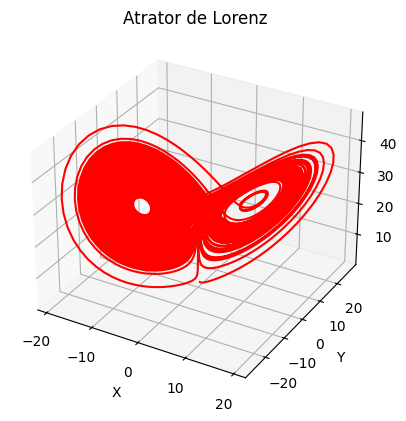
\includegraphics[width=\textwidth]{relatorio/img/plotvaratrator.png}
        \caption{Atrator com $1 \times 10^4$ pontos com valores com variação}
        \label{fig:imagngfem2}
    \end{subfigure}
    \caption{Comparação entre atratores}
    \label{fig:duas_imajygens}
\end{figure}

Principais diferenças:
\begin{itemize}
    \item \textbf{Vórtices:} No primeiro gráfico, os vórtices parecem mais
          preenchidos e definidos, enquanto no segundo gráfico, os vórtices são
          menos
          preenchidos, com espaços mais visíveis entre as linhas de trajetória.

    \item \textbf{Distribuição das Trajetórias: }No primeiro gráfico, as
          trajetórias cobrem mais uniformemente o espaço do atrator. No segundo
          gráfico,
          as trajetórias são mais espaçadas.
\end{itemize}

\begin{figure}[H]
    \centering
    \begin{subfigure}{1.0\textwidth}
        \centering
        \includegraphics[width=\textwidth]{relatorio/img/spline.png}
        \caption{\textit{Spline} cúbica com valores inicias originais}
        \label{fig:spline-original}
    \end{subfigure}
    \vfill
    \begin{subfigure}{1.0\textwidth}
        \centering
        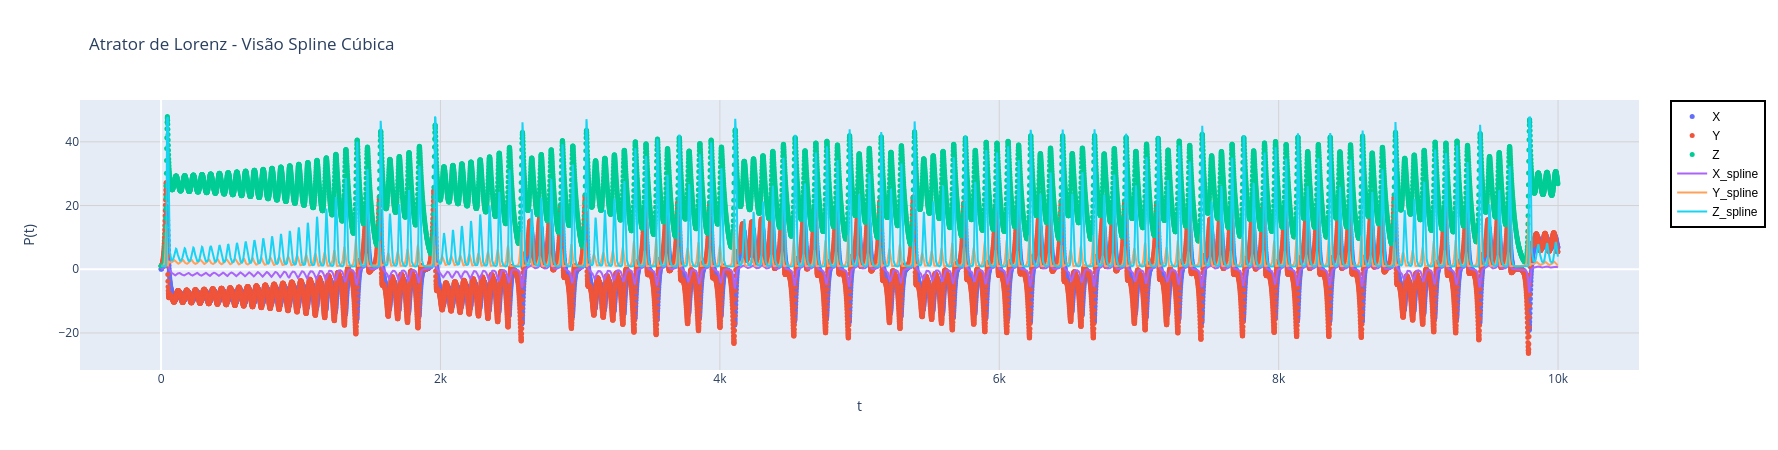
\includegraphics[width=\textwidth]{relatorio/img/plotvarspline.png}
        \caption{\textit{Spline} cúbica com valores inicias com variação}
        \label{fig:spline-va}
    \end{subfigure}
    \caption{Comparação entre \textit{splines} cúbicas}
    \label{fig:comparacao-splines}
\end{figure}

\begin{itemize}
    \item \textbf{X\_spline (linha roxa):}
          \begin{itemize}
              \item \textbf{0k a 2.5k: }O gráfico 01 mostra flutuações significativas com picos altos e vales profundos. O gráfico 02 mostra que essas flutuações são mais suavizadas e menos intensas.
              \item \textbf{2.5k a 5k: }O gráfico 01 mostra flutuações intensas, mas elas estão começando a suavizar. O gráfico 02 mostra a suavização com picos e vales menos marcados.
              \item \textbf{7.5k a 10k:} O gráfico 01 mostra que as flutuações são claramente menores. A linha mostrada no gráfico 02 permanece quase inalterada e apresenta pequenas variações.
          \end{itemize}
    \item \textbf{Y\_spline (linha laranja):}
          \begin{itemize}
              \item \textbf{0k a 2.5k: }O gráfico 01 mostra variações comuns, mas não tão extensas quanto X\_spline. O gráfico 02 mostra que as variações são mais difusas e menos intensas.
              \item \textbf{2.5k a 5k: }O gráfico 01 mostra que as variações são persistentes e marcantes. O gráfico 02 mostra que as variações são menos marcantes e mais suaves.
              \item \textbf{7.5k a 10k:}O gráfico 01 mostra que as variações são espaçadas e mínimas. O gráfico 02 mostra que a suavização é ainda maior.
          \end{itemize}
    \item \textbf{Z\_spline (linha ciano):}
          \begin{itemize}
              \item \textbf{0k a 2.5k: }: O gráfico 01 mostra flutuações mais espaçadas e menores. As variações são ainda menos evidentes quase no gráfico 02. 
              \item \textbf{2.5k a 5k: } O gráfico 01 mostra flutuações mais espaçadas e de menor amplitude. O gráfico 02 mostra que as variações são quase lineares e têm uma amplitude significativa. 
              \item \textbf{7.5k a 10k:}A linha no gráfico 01 é quase linear. O gráfico 02 mostra que a linha permanece estável e apresenta poucas variações.
          \end{itemize}
\end{itemize}

\begin{figure}[H]
    \centering
    \begin{subfigure}{1.0\textwidth}
        \centering
        \includegraphics[width=\textwidth]{relatorio/img/mmq.png}
        \caption{MMQ com valores inicias originais}
        \label{fig:mmq-original}
    \end{subfigure}
    \vfill
    \begin{subfigure}{1.0\textwidth}
        \centering
        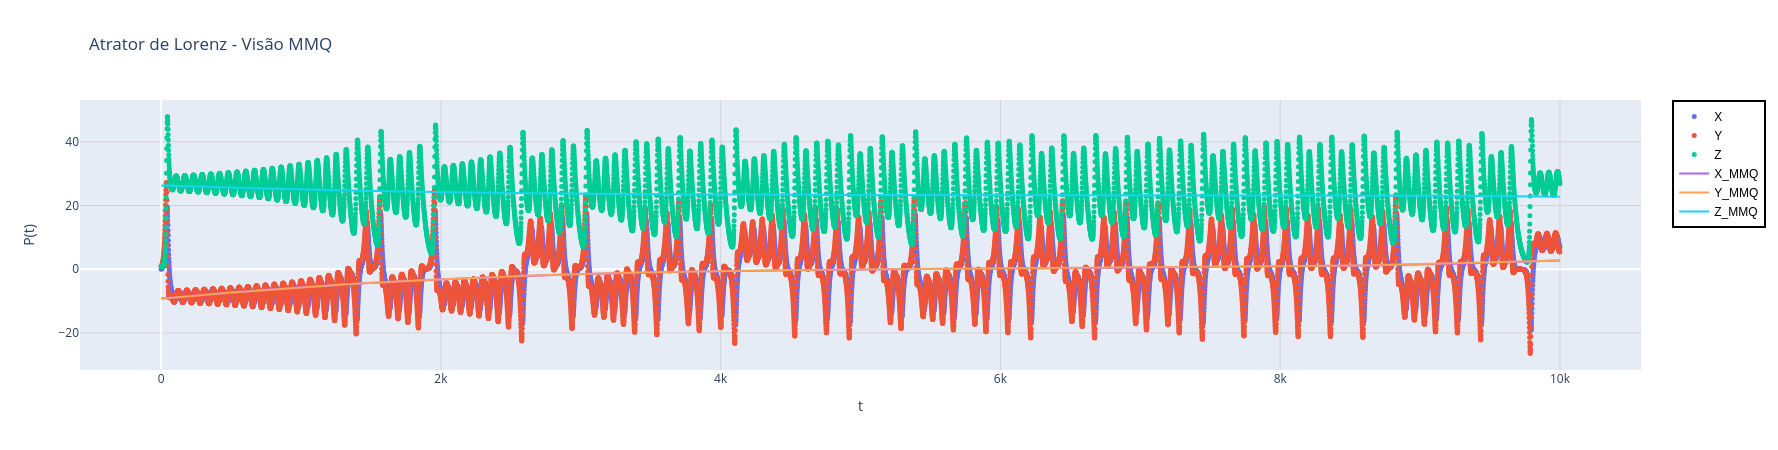
\includegraphics[width=\textwidth]{relatorio/img/plotvarmmq.png}
        \caption{MMQ com valores iniciais com variação}
        \label{fig:mmq-var}
    \end{subfigure}
    \caption{Comparação entre MMQ}
    \label{fig:comparacao-mmq}
\end{figure}

As principais diferenças estão listadas a seguir:
\begin{itemize}
    \item \textbf{X\_MMQ (linha roxa):}
          \begin{itemize}
              \item \textbf{0k a 2.5k: }No gráfico 01, apresentam-se grandes oscilações com picos altos e vales profundos. No gráfico 02, as oscilações são menos intensas e mais suaves.
              \item \textbf{2.5k a 5k: }No gráfico 01, as oscilações são significativas, mas começam a suavizar. No gráfico 02, a suavização é mais evidente, com picos e vales menos acentuados.
              \item \textbf{7.5k a 10k:} No gráfico 01, as oscilações são visivelmente menores. No gráfico 02, a linha é quase estável, com mínimas variações.
          \end{itemize}
    \item \textbf{Y\_MMQ (linha laranja):}
          \begin{itemize}
              \item \textbf{0k a 2.5k:} No gráfico 01, variações frequentes, com menor amplitude que X\_MMQ. No gráfico 02, as variações são menos intensas e mais espaçadas.
              \item \textbf{2.5k a 5k:} No gráfico 01, variações constantes. No gráfico 02, as variações são mais suaves e menos intensas.
              \item \textbf{5k a 7.5k:} No gráfico 01, as variações estão estabilizando. No gráfico 02, a estabilização é mais evidente, com oscilações menos pronunciadas.
              \item \textbf{7.5k a 10k:} No gráfico 01, as variações tornam-se quase inexistentes, com flutuações mínimas. No gráfico 02, a linha torna-se praticamente estável, com variações muito pequenas e quase lineares.
          \end{itemize}
    \item \textbf{Z\_MMQ (linha ciano):}
          \begin{itemize}
              \item \textbf{0k a 2.5k:} No gráfico 01, flutuações menores e espaçadas. No gráfico 02, as flutuações são menos pronunciadas, quase lineares.
              \item \textbf{2.5k a 5k:} No gráfico 01, menor amplitude e espaçadas. No gráfico 02, as variações são quase lineares, com amplitude reduzida.
              \item \textbf{5k a 7.5k:} No gráfico 01, flutuações menores e espaçadas. No gráfico 02, as variações são quase inexistentes, quase lineares.
              \item \textbf{7.5k a 10k:} No gráfico 01, as flutuações são praticamente inexistentes, com variações mínimas. No gráfico 02, a linha torna-se praticamente estável, com oscilações quase imperceptíveis e lineares.
          \end{itemize}
\end{itemize}

\end{itemize}

\newpage
\bibliographystyle{plain}
\bibliography{biblio}
\end{document}
